\chapter{Theoretischer Hintergrund}
\section{E-Learning und digitale Wissensvermittlung}
E-Learning stellt eine neue Lernumgebung dar, die durch den Einsatz von digitalen Medien und Technologien die Wissensvermittlung unterstützt. Es ermöglicht den Lernenden, unabhängig von Zeit und Ort zu lernen und bietet eine Vielzahl von Lernmaterialien und -methoden. Durch den Einsatz von E-Learning können Lernende ihr Wissen effizienter und flexibler erweitern und vertiefen. Dieser Ansatz hat in den letzten Jahren an Bedeutung gewonnen und wird zunehmend in Bildungseinrichtungen und Unternehmen eingesetzt. So fördert E-Learning die Selbstorganisation, kritisches Denken und die Fähigkeit zur Problemlösung der Lernenden. %(Quelle: https://www.researchgate.net/profile/Moradeke-Adewumi/publication/266603233_E-Learning_and_Its_Effects_on_Teaching_and_Learning_in_a_Global_Age/links/62052191634ff774f4c0a84b/E-Learning-and-Its-Effects-on-Teaching-and-Learning-in-a-Global-Age.pdf, Seite 1 f.). 
Zudem ermöglicht E-Learning eine individuelle Anpassung des Lernprozesses an die Bedürfnisse und Präferenzen der Lernenden.
Der Begriff "E-Learning" umfasst verschiedene Formen des elektronisch unterstützten Lernens, darunter Online-Kurse, Webinare, virtuelle Klassenzimmer und interaktive Lernplattformen. Diese Methoden bieten eine interaktive und dynamische Lernumgebung, die traditionelle Lehrmethoden ergänzt und in vielen Fällen ersetzt. Eine der größten Stärken des E-Learnings liegt in seiner Flexibilität: Lernende können in ihrem eigenen Tempo arbeiten und auf eine Vielzahl von Ressourcen zugreifen, die von Texten und Videos bis hin zu interaktiven Simulationen reichen.
Ein weiterer wesentlicher Vorteil des E-Learnings ist die Möglichkeit der kontinuierlichen Aktualisierung und Erweiterung von Lerninhalten. Durch den Einsatz von Learning Management Systems (LMS) können Bildungsanbieter Inhalte schnell und effizient aktualisieren und an neue wissenschaftliche Erkenntnisse oder technologische Entwicklungen anpassen. Diese Systeme ermöglichen es auch, den Lernfortschritt zu überwachen und gezielte Unterstützung anzubieten, was zu einer effektiveren Lernkontrolle und -steuerung führt.
E-Learning bietet zudem die Möglichkeit der Vernetzung und Zusammenarbeit zwischen Lernenden. Durch Foren, Chats und Videokonferenzen können Lernende miteinander in Kontakt treten, sich austauschen und gemeinsam an Projekten arbeiten. Diese sozialen Interaktionen fördern nicht nur das Lernen, sondern auch wichtige soziale Kompetenzen und Teamfähigkeit.
Ein weiterer Aspekt der digitalen Wissensvermittlung ist die Möglichkeit der Personalisierung. Adaptive Lernsysteme passen sich den individuellen Bedürfnissen und Lernstilen der Lernenden an, indem sie deren Fortschritte analysieren und darauf basierend maßgeschneiderte Lernwege vorschlagen. Diese personalisierte Herangehensweise maximiert die Effizienz des Lernprozesses und stellt sicher, dass die Lernenden die für sie relevanten Inhalte in der optimalen Reihenfolge und Tiefe bearbeiten können.
Zusammenfassend lässt sich sagen, dass E-Learning und digitale Wissensvermittlung eine bedeutende Transformation im Bildungswesen darstellen. Sie bieten flexible, effiziente und personalisierte Lernmöglichkeiten, die den Lernenden helfen, ihre Ziele effektiver zu erreichen. Durch die kontinuierliche Weiterentwicklung und Integration neuer Technologien wird E-Learning auch in Zukunft eine zentrale Rolle in der Bildung spielen und zur Verbesserung der Lernprozesse und Lernergebnisse beitragen.

E-Learning stellt eine neue Lernumgebung dar, die durch den Einsatz von digitalen Medien und 
Technologien die Wissensvermittlung unterstützt. Es ermöglicht den Lernenden, unabhängig von Zeit und 
Ort zu lernen und bietet eine Vielzahl von Lernmaterialien und -methoden. %(Quelle:) 
Durch den Einsatz von E-Learning können Lernende ihr Wissen effizienter und flexibler erweitern und vertiefen. %(Quelle:) 
Dieser Ansatz hat in den letzten Jahren an Bedeutung gewonnen und wird zunehmend in 
Bildungseinrichtungen und Unternehmen eingesetzt. So fördert E-Learning die Selbstorganisation, kritisches
Denken oder die Fähigkeit zur Problemlösung der Lernenden. 

\section{Didaktische Konzepte für die Wissensquiz-Erstellung}
Die Erstellung von Wissensquizzen erfordert eine sorgfältige Planung und Umsetzung, um die Lernziele effektiv zu erreichen.
Dabei spielen verschiedene didaktische Konzepte eine wichtige Rolle, um sicherzustellen, dass die Quizfragen relevant, anspruchsvoll und motivierend sind.
Für die Gestaltung von Schulungsartefakten
hat sich in der Wissenschaft mit dem „\ac{ADDIE}“-Modell ein strukturiertes
Vorgehensmodell etabliert, welches den gesamten Entwicklungsprozess von der Analyse über das Design und die Implementierung bis hin zur Evaluation umfasst.
Aus diesem Grund wird im Folgenden das \ac{ADDIE}-Modell vorgestellt und erläutert, wie es für die Erstellung von Wissensquizzen eingesetzt werden kann (siehe Abb. \ref{fig:mondrian}).
\footcite[Vgl.][1805]{nadiyahDevelopmentOnlineProject2015}
\begin{figure}[H]
    \centering
    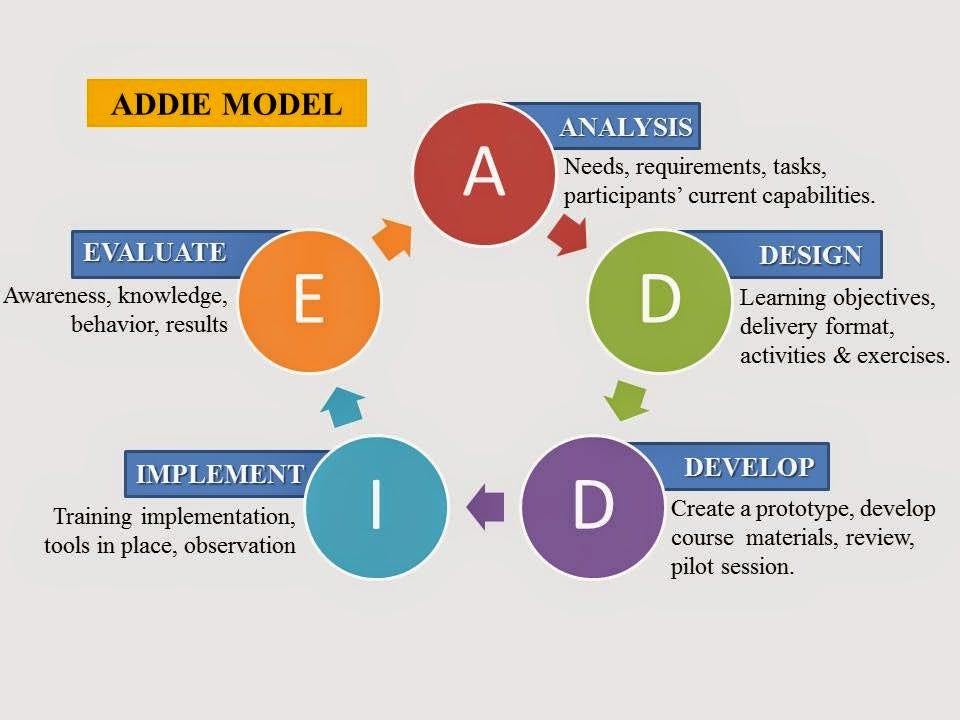
\includegraphics[width=1.0\linewidth]{graphics/addie_model.jpg}
    \caption[Das \acs{ADDIE}-Modell im Überblick.]{Das \ac{ADDIE}-Modell im Überblick.\protect\footnotemark}
    \label{fig:mondrian}
\end{figure}
\footnotetext{Enthalten in: \cite[352]{kuzminskaIVEFFECTIVEMETHODS2017}}
Die erste Phase im \ac{ADDIE}-Modell sieht die Durchführung einer Bedarfsanalyse vor, um die Lernziele und -bedürfnisse der Zielgruppe korrekt erfassen zu können.
Als Möglichkeit hierfür wird von Allen 2006 unter anderem die Erstellung einer Aufgabenliste vorgeschlagen, welche für
den Vergleich mit den Fähigkeiten und Kenntnissen der Zielgruppe genutzt werden kann.
\footcite[Vgl.][436]{allenOverviewEvolutionADDIE2006}
Hierbei ist ein besonderes Augemerk auf die Unterschiede zwischen dem gegenwärtigen Ist- und dem gewünschten Soll-Zustand in Bezug auf das vorhandene Wissen zu legen.
\footcite[Vgl.][436]{allenOverviewEvolutionADDIE2006}
Auf dieser Basis können schließlich Anforderungen an das zu erstellende Schulungsartefakt abgeleitet werden.
Für den vorliegenden Anwendungsfall der Quizerstellung in Moodle bedeutet dies, dass die Sekretärinnen und Sekretären
der Fakultät als Zielgruppe zu identifizieren sind und daher die Fragen entsprechend deren Kenntnisstand und Bedürfnissen gestaltet werden müssen.
So ist bspw. von Fragen, welche bloße Fakten und Definitionen abfragen, ebenso abzusehen wie von Fragen, welche
primär IT-administratives Fachwissen erfordern. Eine Zusammensetzung von Fragen, welche
einerseits theoretischer Natur sind und andererseits auch praktische Anwendungsfälle abbilden, scheint hingegen sinnvoll.
Letzteres könnte bspw. durch die Einbindung von Fallbeispielen oder Praxisübungen erfolgen, während für den
theoretischen Teil komplexere Fragen, welche ein tieferes Verständnis von Rapla erfordern, genutzt werden könnten.

Den zweiten Schritt im \ac{ADDIE}-Modell bildet die Design-Phase, in welcher eine detaillierter Plan an Anweisungen und Inhalten für das zu erstellende Schulungsartefakt erstellt wird.
Hierunter fällt auch die Auswahl entsprechender Lehrmethoden und -medien sowie eine kritische Überprüfung aktuell vorliegender Materialien.
\footcite[Vgl.][436]{allenOverviewEvolutionADDIE2006} 
Gemäß xx ist in dieser Phase insbesondere darauf zu achten, dass anhand des aufgestellten Plans letztlich eine präzise Abbildung der festgelegten Ziele erfolgt.
Ebenfalls Gegenstand dieser Phase ist die Entwicklung konzeptioneller Grundlagen für das zu erstellende Artefakt, worunter
bspw. die Entwicklung oder die Implementierung eines geeigneten Bildungsinformationsmanagementsystems fallen könnte.
\footcite[Vgl.][436]{allenOverviewEvolutionADDIE2006}
Von besonderer Relevanz
ist in dieser Phase auch die Taxonomie nach Bloom, die eine Klassifizierung von Lernzielen und -aktivitäten ermöglicht.
\dots

In der dritten Phase des \ac{ADDIE}-Modells erfolgt die Implementierung des eigentlichen Schulungsartefakts.
Für den vorliegenden Anwendungsfall fällt hierunter die tatsächliche Erstellung des Wissensquiz in Moodle.
Als alternative Entwicklungsinhalte könnten laut Allen 2006 hierunter auch Videos, Simulationen oder interaktive Lernmaterialien fallen.
\footcite[Vgl.][437]{allenOverviewEvolutionADDIE2006}
Ebenso ist die Revision des erstellten Schulungsartefakts in dieser Phase von Bedeutung, um sicherzustellen, dass die erstellten Inhalte den zuvor festgelegten Anforderungen entsprechen.
\footcite[Vgl.][437]{allenOverviewEvolutionADDIE2006}

In der vierten Phase wird das erstellte Schulungsartefakt in den operativen
Betrieb überführt. Ebenso ist hierbei die Sammlung von ersten Rückmeldungen
der Nutzerinnen und Nutzer von Bedeutung, um das Artefakt ggf. nochmals
anpassen zu können bzw. eine Grundlage für die fünfte Phase des \ac{ADDIE}-Modells zu schaffen.

Die fünfte und letzte Phase des \ac{ADDIE}-Modells bildet die Evaluation des erstellten Schulungsartefakts.
Hierbei wird kritisch überprüft, ob die erstellten Inhalte mit den zuvor festgelegten Ziele übereinstimmen und das Artefakt auf die Anforderungen der Zielgruppe abgestimmt ist.
\footcite[Vgl.][437]{allenOverviewEvolutionADDIE2006}
Ebenfalls fallen unter diese Phase Überlegungen zur Effektivität der erstellten Lösung.
\footcite[Vgl.][2]{constancioExtendedADDIEModel2018}

Insgesamt wird das \ac{ADDIE}-Modell in der Forschungsliteratur als ein effektives und strukturiertes Vorgehensmodell für die Erstellung von Schulungsartefakten angesehen.
So heben bspw. Drljača u. a. 2017 das hohe Maß an Flexibilität als Vorteil hervor, da das Modell auf verschiedene Bildungs- und Trainingsbedarfe anwendbar ist.
\footcite[Vgl.][247]{drljacaADDIEModelDevelopment2017}
Als großer Kritikpunkt hingegen wird angesehen, dass vorausgesetzt wird, dass vorab bereits
alle Anforderungen bekannt sind und sich diese im Projektverlauf nicht mehr ändern.

Als Beispiele hierfür werden von Drljača u. a. 2017 sowohl
Schwierigkeiten bzgl. der Integration von guten Ideen, welche
im Projektverlauf entstehen können, als auch Probleme im Umgang
mit unerwarteten Fehlern genannt.
\footcite[Vgl.][246]{drljacaADDIEModelDevelopment2017}


\section{Zertifizierungen als Erfolgsfaktor}
Zertifizierungen spielen eine zentrale Rolle in der beruflichen Weiterbildung und Entwicklung. Sie bieten nicht nur einen formalen Nachweis über die Teilnahme und den erfolgreichen Abschluss eines Trainings, sondern vermitteln auch Vertrauen in die erworbenen Fähigkeiten und Kenntnisse. Dieser Abschnitt untersucht die Bedeutung von Zertifizierungen in Trainingsprogrammen, die Arten von Aufgaben, die für deren Erlangung gelöst werden müssen, und die Auswirkungen auf die Karriereentwicklung. % (Quelle: https://www.mdpi.com/2227-7102/12/8/525 Seite 1 f.)

Funktionen und Vorteile von Zertifizierungen
Validierung von Fähigkeiten und Wissen: Zertifizierungen dienen als offizieller Nachweis für die erworbenen Kenntnisse und Fähigkeiten in einem bestimmten Bereich. Sie bieten eine objektive Bestätigung, dass der Teilnehmer die erforderlichen Kompetenzen erfolgreich erworben hat. % (Quelle:https://www.researchgate.net/publication/225083565_Employability_Developing_a_framework_for_policy_analysis Seite 4) 

Erhöhung der Arbeitsplatzchancen: In vielen Branchen und Berufsfeldern sind Zertifizierungen ein wichtiger Faktor bei der Einstellung und Beförderung. Arbeitgeber sehen in zertifizierten Kandidaten oft eine geringere Einarbeitungszeit und ein höheres Maß an Fachkompetenz. So zeigen Studien, dass Personen mit Zertifikaten höhere Chancen haben, höhere Gehälter zu erhalten als Personen ohne Zertifizierung. %(Quelle:https://d1wqtxts1xzle7.cloudfront.net/110511099/ARTICULO_Qualifications_and_Certificates_v_PraKnowledge_and_Experience_Is_There_a_Winner_2019_YORKYS-libre.pdf?1705421798=&response-content-disposition=inline%3B+filename%3DQualifications_and_Certificates_v_Practi.pdf&Expires=1720369139&Signature=GI5mIM62xovQEHeWaavAniL5-L37~FH7siRjZ~yxuKz-s402q~OLldz0FfRAcdfpWe41yOtNWWdTLRtOeJPLava6uBi0TjvQnG0YBoiyAnGW~Or0uCnlw5KZLdRb2~WN05U7xhEmr3ISPtvrmZwJxCzL56KNl35oMu1lIJzHG8-eXWz5D~XSpOA72FCbrY6F-3UzHc-emOS0iuXS8q398nisRUefEO8ifhEpLME9A1Jfoc-ziaOLpUsTXOPwLzVvbK6RQD1bqCMERSw7lJPTIoxdKF~RI~7auVblkHFQ2bhTJK4aaQLj9BoYnHloo3nyg5ZTpj0L1XF1FHl5IVqVaQ__&Key-Pair-Id=APKAJLOHF5GGSLRBV4ZA Seite 7)

Selbstvertrauen und Motivation: Der Erhalt einer Zertifizierung kann das Selbstbewusstsein der Teilnehmer stärken und sie motivieren, weiter an ihrer beruflichen Entwicklung zu arbeiten. Es stellt eine greifbare Anerkennung ihrer Bemühungen und ihres Engagements dar. % (Quelle: https://www.mdpi.com/2227-7102/12/8/525 Seite 1)

Standardisierung und Vergleichbarkeit: Zertifizierungen tragen zur Standardisierung von Fähigkeiten und Wissensniveaus bei, indem sie klare Anforderungen und Bewertungskriterien festlegen. Dies erleichtert den Vergleich von Qualifikationen zwischen verschiedenen Individuen und Organisationen.

Arten von Aufgaben zur Erlangung von Zertifizierungen
Um eine Zertifizierung zu erlangen, müssen Teilnehmer in der Regel eine Reihe von Aufgaben und Prüfungen erfolgreich absolvieren. Diese Aufgaben sind darauf ausgelegt, die Beherrschung der vermittelten Inhalte und Fähigkeiten zu überprüfen. Zu den häufigsten Aufgabenarten gehören:

Theoretische Prüfungen: Diese Tests überprüfen das Verständnis der theoretischen Grundlagen des jeweiligen Fachgebiets. Sie bestehen oft aus Multiple-Choice-Fragen, Kurzantworten oder Essay-Fragen.

Praktische Prüfungen: Praktische Prüfungen verlangen von den Teilnehmern, bestimmte Aufgaben oder Projekte durchzuführen, die direkt mit den erworbenen Fähigkeiten in Zusammenhang stehen. Diese können Laborarbeiten, Programmieraufgaben oder Fallstudien umfassen.

Projektarbeiten: In vielen Zertifizierungsprogrammen müssen Teilnehmer eigenständige Projekte bearbeiten, die ihr Wissen und ihre Fähigkeiten in realen Szenarien anwenden. Diese Projekte werden oft dokumentiert und präsentiert.

Simulationen und Fallstudien: Diese Methoden testen die Fähigkeit der Teilnehmer, komplexe Probleme zu analysieren und Lösungen zu entwickeln. Simulationen und Fallstudien spiegeln häufig reale berufliche Herausforderungen wider.

Auswirkungen auf die Karriereentwicklung:
Zertifizierungen haben weitreichende Auswirkungen auf die Karriereentwicklung. Sie ermöglichen es den Teilnehmern, sich von Mitbewerbern abzuheben und ihre Fachkompetenz nachzuweisen. Folgende Aspekte sind besonders hervorzuheben:

Karrieresprungbrett: Zertifizierungen können als Sprungbrett für höhere Positionen und verantwortungsvollere Aufgaben dienen. Viele Führungskräftepositionen setzen bestimmte Zertifizierungen voraus.

Netzwerkmöglichkeiten: Trainingsprogramme und Zertifizierungen bieten oft Möglichkeiten zum Netzwerken mit anderen Fachleuten und Experten in der Branche. Dies kann zu neuen beruflichen Kontakten und Chancen führen.

Kontinuierliche Weiterbildung: Zertifizierungen fördern die Kultur des lebenslangen Lernens. Teilnehmer bleiben motiviert, ihre Kenntnisse und Fähigkeiten kontinuierlich zu aktualisieren und zu erweitern, um den Anforderungen des sich ständig verändernden Arbeitsmarktes gerecht zu werden.

Trotz der zahlreichen Vorteile von Zertifizierungen gibt es auch kritische Stimmen, die die zunehmende Bedeutung und den inflationären Einsatz von Zertifikaten hinterfragen. Diese Kritikpunkte sind wichtig, um ein ausgewogenes Bild von der Rolle und dem Wert von Zertifizierungen in der beruflichen Weiterbildung zu erhalten.

Inflation und Qualitätsverlust:
Ein Hauptkritikpunkt ist die Inflation von Zertifikaten. In vielen Bereichen werden Zertifizierungen für eine Vielzahl von Themen und Fähigkeiten angeboten, oft ohne strenge Qualitätskontrollen. Dies führt zu einer Entwertung der Zertifikate, da der Markt mit einer Vielzahl von teilweise minderwertigen Zertifikaten überschwemmt wird. Arbeitgeber können Schwierigkeiten haben, den tatsächlichen Wert eines Zertifikats zu erkennen, wenn sie nicht sicher sein können, welche Standards bei der Zertifizierung eingehalten wurden.

Oberflächliches Wissen statt tiefgreifender Kompetenzen:
Ein weiterer Kritikpunkt betrifft die Art und Weise, wie Zertifizierungen strukturiert sind. Oft liegt der Fokus auf dem Erreichen von Prüfungsanforderungen und dem Erhalt des Zertifikats, anstatt auf dem tiefgreifenden Verständnis und der Anwendung des Wissens. Teilnehmer könnten lediglich darauf trainiert werden, Prüfungen zu bestehen, ohne die Fähigkeit zu entwickeln, das Gelernte effektiv in der Praxis anzuwenden. Dies führt zu einer Diskrepanz zwischen zertifizierten Kenntnissen und tatsächlicher beruflicher Kompetenz. %(Quelle: https://d1wqtxts1xzle7.cloudfront.net/110511099/ARTICULO_Qualifications_and_Certificates_v_PraKnowledge_and_Experience_Is_There_a_Winner_2019_YORKYS-libre.pdf?1705421798=&response-content-disposition=inline%3B+filename%3DQualifications_and_Certificates_v_Practi.pdf&Expires=1720369139&Signature=GI5mIM62xovQEHeWaavAniL5-L37~FH7siRjZ~yxuKz-s402q~OLldz0FfRAcdfpWe41yOtNWWdTLRtOeJPLava6uBi0TjvQnG0YBoiyAnGW~Or0uCnlw5KZLdRb2~WN05U7xhEmr3ISPtvrmZwJxCzL56KNl35oMu1lIJzHG8-eXWz5D~XSpOA72FCbrY6F-3UzHc-emOS0iuXS8q398nisRUefEO8ifhEpLME9A1Jfoc-ziaOLpUsTXOPwLzVvbK6RQD1bqCMERSw7lJPTIoxdKF~RI~7auVblkHFQ2bhTJK4aaQLj9BoYnHloo3nyg5ZTpj0L1XF1FHl5IVqVaQ__&Key-Pair-Id=APKAJLOHF5GGSLRBV4ZA Seite 4 f.)

Kosten und Zugang:
Zertifizierungen sind oft mit hohen Kosten verbunden, sowohl in Bezug auf die Teilnahmegebühren als auch auf die Vorbereitungsmaterialien und -kurse. Dies kann zu einer Barriere für viele Fachleute werden, insbesondere für diejenigen, die sich die finanziellen Ausgaben nicht leisten können. Infolgedessen können Zertifizierungen zu einer Art von Exklusivität führen, bei der nur bestimmte Individuen die Möglichkeit haben, ihre Qualifikationen formell zu bestätigen. %(Quelle: https://www.mdpi.com/2227-7102/12/8/525 Seite 2 f.)

Alternativen zu Zertifizierungen:
In vielen Bereichen gewinnen alternative Nachweise an Bedeutung. Dazu gehören praktische Erfahrung oder Projektportfolios, die oft ein besseres Bild von den tatsächlichen Fähigkeiten und der beruflichen Eignung eines Kandidaten vermitteln. Unternehmen beginnen zunehmend, auf diese alternativen Bewertungsmethoden zu setzen, um die Eignung eines Kandidaten für eine bestimmte Position zu bestimmen.

Zertifizierungen in Trainingsprogrammen bieten eine wertvolle Möglichkeit zur beruflichen Weiterbildung und Qualifizierung. Sie dienen als formale Bestätigung von erworbenen Fähigkeiten und Wissen, erhöhen die Arbeitsplatzchancen, stärken das Selbstvertrauen und fördern die Standardisierung und Vergleichbarkeit von Qualifikationen. Als Karrieresprungbrett eröffnen sie neue berufliche Möglichkeiten, bieten Netzwerkmöglichkeiten und unterstützen die Kultur des lebenslangen Lernens.

Trotz einiger kritischer Aspekte, wie der Inflation von Zertifikaten und potenziellen Qualitätsverlusten, bleibt der positive Einfluss von Zertifizierungen unbestritten. Sie stellen eine greifbare Anerkennung für die Bemühungen und das Engagement der Teilnehmer dar und motivieren zur kontinuierlichen beruflichen Entwicklung. Auch wenn es wichtig ist, die Grenzen und Herausforderungen von Zertifizierungen zu erkennen, überwiegen die Vorteile für viele Fachleute und Arbeitgeber. 

Insgesamt tragen Zertifizierungen wesentlich zur beruflichen Weiterentwicklung bei und bieten einen klaren Nachweis über die erworbenen Kompetenzen. Durch ein ausgewogenes Verständnis ihrer Vor- und Nachteile können sie effektiv in den individuellen Karriereweg integriert werden, um langfristigen beruflichen Erfolg zu unterstützen.

\section{Gestaltung von Usability-Tests}
Usability-Tests sind ein entscheidendes Instrument zur Evaluierung der Benutzerfreundlichkeit und Effektivität einer Anwendung oder eines Systems (https://journals.sagepub.com/doi/abs/10.1177/1541931213571042 Seite 187). 
Sie bieten wertvolle Einblicke in das Nutzerverhalten und helfen dabei, Schwachstellen zu identifizieren sowie Optimierungspotenziale aufzuzeigen.(https://onlinelibrary.wiley.com/doi/epdf/10.1002/9781118976005.ch14 Seite 257) 
Die Gestaltung von Usability-Tests erfordert eine sorgfältige Planung und Durchführung, um aussagekräftige und verlässliche Ergebnisse zu erzielen.

\begin{enumerate}
    \item \textbf{Ziele und Hypothesen:}

Der erste Schritt bei der Gestaltung eines Usability-Tests besteht darin, klare Ziele und Hypothesen zu definieren. Diese sollten die spezifischen Aspekte der Benutzererfahrung adressieren, die getestet werden sollen. Beispiele für solche Ziele können die Überprüfung der Verständlichkeit der Benutzeroberfläche, die Effizienz der Navigation oder die Zufriedenheit der Nutzer mit bestimmten Funktionen sein. Die Hypothesen sollten konkrete Annahmen über das Nutzerverhalten und die Leistung der Anwendung beinhalten, die im Test überprüft werden sollen.

    \item \textbf{Testpersonen auswählen:}

Die Auswahl der Testpersonen ist ein weiterer wichtiger Schritt. Die Teilnehmer sollten eine repräsentative Stichprobe der tatsächlichen Nutzer darstellen. Dabei ist es wichtig, verschiedene Nutzergruppen zu berücksichtigen, um ein breites Spektrum an Perspektiven und Erfahrungen zu erfassen. Faktoren wie Alter, Geschlecht, technisches Verständnis und spezifische Nutzeranforderungen spielen hierbei eine Rolle.


    \item \textbf{Testmethoden und Szenarien:}

Usability-Tests können mit unterschiedlichen Methoden durchgeführt werden, die je nach den Testzielen variieren. Zu den gängigen Methoden gehören:

Moderierte Tests: Ein Moderator führt die Testpersonen durch vorab definierte Aufgaben und stellt gezielte Fragen, um deren Gedankenprozesse und Reaktionen zu verstehen.

Unmoderierte Tests: Die Teilnehmer führen die Aufgaben eigenständig durch, während ihre Interaktionen aufgezeichnet werden.

Remote-Tests: Diese werden online durchgeführt, wodurch eine größere und geografisch diversifizierte Teilnehmergruppe erreicht werden kann.

Die Testmethoden werden durch spezifische Szenarien ergänzt, die typische Nutzungssituationen der Anwendung simulieren. Diese Szenarien sollten realistisch und relevant für die Zielgruppe sein, um aussagekräftige Ergebnisse zu gewährleisten.


    \item \textbf{Datenerhebung und Analyse:}

Während des Tests werden verschiedene Arten von Daten erhoben, darunter:

Qualitative Daten: Beobachtungen, Kommentare und offene Feedbacks der Teilnehmer. Diese Daten liefern Einblicke in die subjektiven Erfahrungen und Meinungen der Nutzer.
Quantitative Daten: Metriken wie die Zeit zur Aufgabenbewältigung, Fehlerraten und Erfolgsmessungen. Diese Daten ermöglichen objektive Vergleiche und statistische Analysen.
Die Datenanalyse erfolgt in mehreren Schritten. Zunächst werden die gesammelten Daten strukturiert und kategorisiert. Anschließend werden sie auf Muster und Auffälligkeiten hin untersucht. Dabei können sowohl einfache deskriptive Statistiken als auch komplexere inferenzstatistische Methoden zur Anwendung kommen.


    \item \textbf{Berichterstellung und Handlungsempfehlungen:}
\end{enumerate}
Die Ergebnisse des Usability-Tests werden in einem umfassenden Bericht dokumentiert. Dieser sollte sowohl die Methodik und die Durchführung des Tests als auch die wesentlichen Erkenntnisse und Schlussfolgerungen beinhalten. Wichtige Elemente des Berichts sind:
Zusammenfassung der wichtigsten Ergebnisse: Eine prägnante Darstellung der zentralen Erkenntnisse.
Detaillierte Ergebnisse: Ausführliche Beschreibungen der beobachteten Probleme und ihrer Auswirkungen auf die Nutzererfahrung.
Visuelle Darstellungen: Grafiken und Diagramme, die die Ergebnisse veranschaulichen und leichter verständlich machen.
Handlungsempfehlungen: Konkrete Vorschläge zur Verbesserung der Benutzerfreundlichkeit, basierend auf den Testergebnissen.

Durch eine sorgfältige Planung und Durchführung von Usability-Tests können wertvolle Erkenntnisse gewonnen werden, die zur Verbesserung der Benutzerfreundlichkeit und somit zum Erfolg einer Anwendung beitragen.
